\subsection{Noise}

A princípio, o "Noise" foi definido como uma primitiva de modelagem de textura para o Pixel Streaming Editor que o Ken Perlin \cite{fractalNoise} propôs, mas a implementação da técnica pode ser reproduzida em outras ferramentas. 

Em um espaço vetorial onde cada ponto para as coordenadas $x,y,z$ são inteiros, cada ponto deste conjunto pode ser associado a um valor "pseudorandom", onde $x, y, z$ são valores gradientes.
Deste modo, deve-se mapear cada sequência ordenada de três inteiros em uma sequencia ordenada de 4 números reais, de modo que:

$[a,b,c,d] = H([x,y,z])$ onde $[a,b,c,d]$ definem a equação com o gradiente $[a,b,c]$ e o valor "d" em $[x,y,z]$. $H()$ seria uma função HASH. 

A partir disso, se [x,y,z] está neste set de inteiros, é definido o $Noise([x,y,z]) = d[x,y,z]$, interpretado como um sinal (apresenta frequência). 

Com estas definições, supondo um vetor aleatório array, e que ele representa um Donut $color = white * Noise(array)$, com a aplicação desta "transformada" foi possível criar essas ondulações no donut com as texturas brancas, de forma aleatória.

\begin{figure}[H]
    \centering
    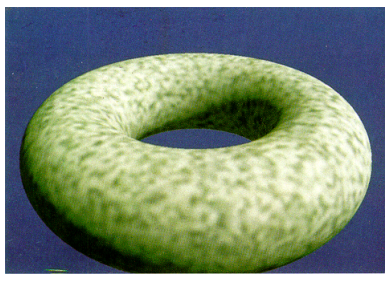
\includegraphics[width=0.4\textwidth]{img/donut.png}
    \caption{Donut com textura Noise aplicada}
    \label{fig:donut_noise}
\end{figure}

$color = Colorful(Noise(k * array))$ outro possível exemplo de aplicação, 

\begin{figure}[H]
    \centering
    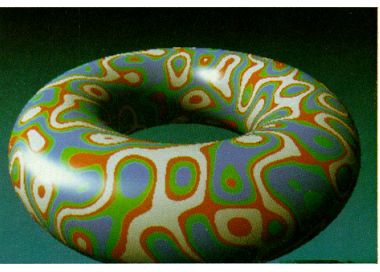
\includegraphics[width=0.4\textwidth]{img/donut2.png}
    \caption{Esfera com textura Noise aplicada}
    \label{fig:sphere_noise}
\end{figure}

\begin{figure}[H]
    \centering
    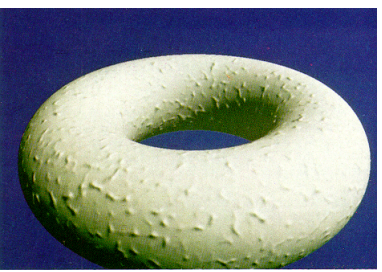
\includegraphics[width=0.4\textwidth]{img/donut3.png}
    \caption{Cubo com textura Noise aplicada}
    \label{fig:cube_noise}
\end{figure}

Outra técnica seria o vetor diferencial do Noise(), que é definido pela taxa de variação instantânea do "ruído" através das três direções, chamados de Dnoise().

A partir desta aplicação fica possível criar outros tipos de perturbação, originando novas superfícies e texturas. 

$$
normal += Dnoise(array)
$$

\begin{figure}[H]
    \centering
    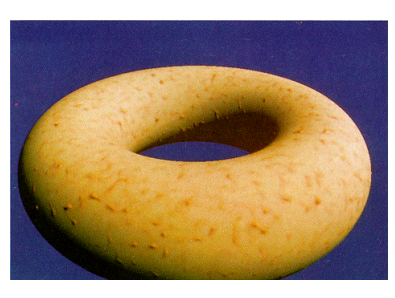
\includegraphics[width=0.4\textwidth]{img/donut4.png}
    \caption{Donut com textura Dnoise aplicada}
    \label{fig:donut_dnoise}
\end{figure}

Como estes cálculos e tecnicas são aplicados em nível de pixel, a frequència de cada pixel é que está sendo utilizada, logo, qualquer frequência de taxa mais alta que não seja desejada é automaticamente removida. 

Exemplo de cálculo com a frequência inversa, aplicando transformações em todos os octetos:

\begin{lstlisting}[language=Python, caption={Pseudocódigo da função turbulence()}]
f=l
while (f < pixel_freq):
  normal + = Dnoise(f * point)
  f*=2 
\end{lstlisting}

O autor descreve uma técnica para simular a aparência de mármore usando a função Noise(). O método parte do princípio de que a aparência do mármore resulta de camadas heterogêneas que foram deformadas por forças turbulentas antes de se solidificarem. A abordagem é, portanto, uma combinação de uma estrutura regular e simples (as camadas) com uma complexa estrutura estocástica (o ruído da turbulência). A base do modelo são as camadas, representadas por uma simples onda senoidal, sin(x). O autor usa a coordenada point[1] como o input para essa função, e o valor resultante é então mapeado para cores através de uma função auxiliar marble\_color(). Para adicionar o realismo das forças turbulentas, o autor introduz uma função turbulence(). Esta função é usada para perturbar a coordenada de entrada x antes que ela seja passada para a onda senoidal. O pseudocódigo que combina esses elementos é o seguinte:

% code
\begin{lstlisting}[language=Python, caption={Pseudocódigo da função turbulence()}]
def marble(point):
  x = point[1] + turbulence(point)
  return marble\_color(sin(x))
\end{lstlisting}

A função turbulence() é, por sua vez, uma soma de ruído em diferentes escalas, um processo que cria um padrão auto-semelhante ou 1/f. O algoritmo para a turbulence() é detalhado como:

\begin{lstlisting}[language=Python, caption={Pseudocódigo da função turbulence()}]
def turbulence(p):
  t = 0
  scale = 1
  while (scale > pixelsize)
    t += abs(Noise(p / scale) * scale)
    scale *= 2
  return t
\end{lstlisting}

Este procedimento garante que a quantidade de ruído adicionada em cada escala seja proporcional ao seu tamanho, resultando na impressão visual de movimento browniano. Além disso, o uso da função abs() em cada iteração assegura que o gradiente da textura tenha limites descontínuos em todas as escalas, o que é interpretado visualmente como fluxo turbulento

\begin{figure}[H]
    \centering
    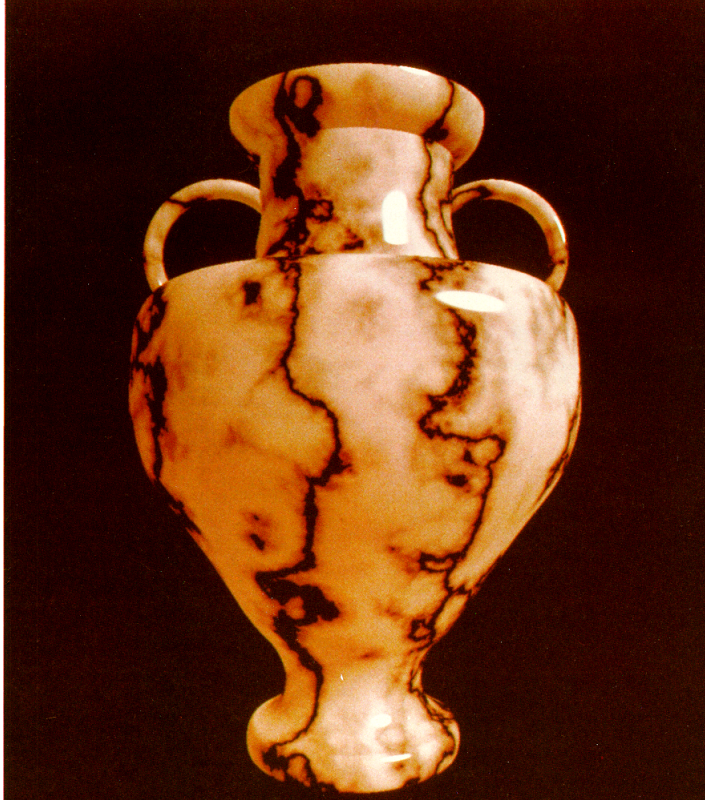
\includegraphics[width=0.4\textwidth]{img/marble.png}
    \caption{Textura de mármore gerada com a função marble()}
    \label{fig:marble_texture}
\end{figure}

\subsubsection{Fractional Brownian Motion no Perlin Noise (or fractal noise)}
Fractional Brownian Motion (fBm) é uma técnica utilizada para gerar texturas e superfícies naturais em computação gráfica, especialmente em simulações de terrenos, nuvens e outros fenômenos naturais. A fBm é uma extensão do conceito de movimento browniano, que descreve o movimento aleatório de partículas em um fluido. Na fBm, esse movimento é caracterizado por uma escala fractal, permitindo a criação de padrões auto-similares em diferentes níveis de detalhe \cite{fractalNoise}.

Para isso, a fBm é construída somando várias camads de ruído Perlin, cada uma com uma frequência e amplitude diferentes. A fórmula geral para calcular a fBm é dada por:

$$
fBm(x, y, z) = \sum_{i=0}^{n-1} amplitude_i \cdot Noise(frequency_i \cdot (x, y, z))
$$


\subsection{Mapeamento de Texturas}

Qualquer função que apresente o domínio entre as dimensôes pode ser considerado uma "função espacial". A partir disso, cada função espacial pode ser interpretada como a representação de um material sólido.

Desta forma, ao avaliar estas funções nos pontos visíveis da superfície de um objeto, é possível obter a textura da superfície, de modo parecido a ter "contornado" o objeto. A textura obtida a partir deste tipo de extração foi tratada como "textura sólida". Este termo foi usado posteriormente para a descrição da variedade de objetos e explicação de outros conceitos.

